\documentclass[tikz, multi=tikzpicture]{standalone}
\usepackage{amsmath}

% --- Colors matching the python script & blog post math ---
\definecolor{Ocol}{HTML}{3273F6}    % Ray Origin (Blue)
\definecolor{Dcol}{HTML}{FF4B4B}    % Ray Direction (Red)
\definecolor{Ccol}{HTML}{109618}    % Sphere Center (Green)
\definecolor{Rcol}{HTML}{990099}    % Radius (Purple)
\definecolor{Acol}{HTML}{FF9900}    % Triangle Vertex A (Orange)
\definecolor{Bcol}{HTML}{0099C6}    % Triangle Vertex B (Light Blue)
\definecolor{Ctri}{HTML}{DD4477}    % Triangle Vertex C (Pink)
\definecolor{Textcol}{HTML}{333333}
\definecolor{Gridcol}{HTML}{E0E0E0}

\usetikzlibrary{calc, intersections, arrows.meta, positioning}

\tikzset{
    >=Stealth,
    font=\sffamily
}

\begin{document}

% ---------------------------------------------------------
% 1. Basic Ray-Sphere Intersection
% ---------------------------------------------------------
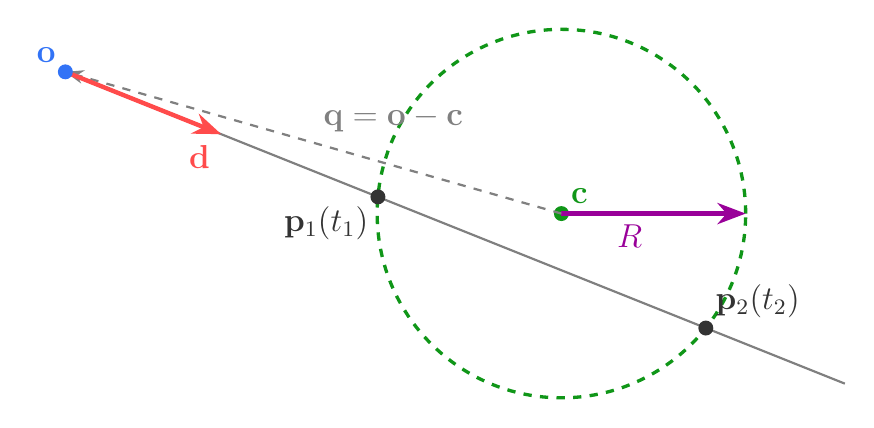
\begin{tikzpicture}[scale=0.9]
    % Grid
    % \draw[step=1, Gridcol, very thin] (0,0) grid (12,8);
    
    % Coordinates
    \coordinate (C) at (8, 4);
    \def\R{2.6}
    \coordinate (O) at (1, 6);
    \coordinate (RayEnd) at (12, 1.6); 

    % Sphere
    \draw[Ccol, very thick, dashed, name path=circle] (C) circle (\R);
    \fill[Ccol] (C) circle (3pt) node[above right, font=\large] {$\mathbf{c}$};

    % Radius
    \draw[->, Rcol, ultra thick] (C) -- ++(0:\R) node[midway, below left, font=\large] {$R$};

    % q vector (o - c)
    \draw[->, gray, thick, dashed] (C) -- (O) node[midway, above right, font=\large] {$\mathbf{q} = \mathbf{o} - \mathbf{c}$};

    % Ray line
    \draw[gray, thick, name path=ray] (O) -- (RayEnd);
    
    % Ray direction vector
    \coordinate (D) at ($(O)!0.2!(RayEnd)$);
    \draw[->, Dcol, ultra thick] (O) -- (D) node[below left, font=\large] {$\mathbf{d}$};

    % Ray Origin
    \fill[Ocol] (O) circle (3pt) node[above left, font=\large] {$\mathbf{o}$};

    % Intersection Points
    \path [name intersections={of=circle and ray, by={p1, p2}}];
    \fill[Textcol] (p1) circle (3pt) node[below left, font=\large] {$\mathbf{p}_1 (t_1)$};
    \fill[Textcol] (p2) circle (3pt) node[above right, font=\large] {$\mathbf{p}_2 (t_2)$};
\end{tikzpicture}

\end{document}